\section{What is survey data?}

Large-scale surveys form the basis for many scientific enquiries which use a sample to investigate some property of the wider population. Examples of these include political polls, workforce participation statistics, disease prevalence, and healthcare utilisation, to name a few. These types of studies typically follow a design known as the complex sample survey (CSS) design. This type of survey design is often taken for granted today as the basic statistical methodology is well-established, but this has not always been the case. For many years, the simple random sample (SRS) design was the default method for collecting data on populations \citep{heeringa2017}. That was until methodological developments on making inference with stratified samples culminated in seminal work by \citet{neyman1934}. Following this, interest in the field grew rapidly, and many new methods for survey design and inference were developed. 

During the second half of the $20^{\text{th}}$ century, methods such as generalised linear models (GLMs) became prominent. However, these centre around the assumption of independently sampled observations, which does not hold true for CSSs. It was during the 1970s and 1980s when methods for appropriately implementing these models with CSSs were developed by survey statisticians \citep{heeringa2017}. This allows for the analysis of CSS data to be divided into two types: (i) descriptive analyses which centre around inferring population statistics i.e., "design-based" analysis, (ii) explanatory analyses which centre around inferring relationships between variables i.e., "model-based" analysis \citep{heeringa2017}.

\section{Design-based inference}

Complex sample surveys aim to describe a target population, which is a finite population of size $N$, where $N$ can range from hundreds of individuals through to billions. Each element $(i = 1, ..., N)$ may theoretically be sampled as part of the survey design. Therefore, CSSs involve taking a sample of size $n$, without replacement, from a finite population of size $N$. This results in a reduction in the variance of any estimated statistics. The factor that the variance is reduced by is known as the finite population correction (FPC) \citep{heeringa2017}:

\begin{align}
\label{eq:fpc}
\text{FPC} = 1 - \frac{n}{N}
\end{align}

Typically, $\frac{n}{N}$ is so small that $\text{FPC} \approx 1$. 

Unlike an SRS, the sampling probability in a CSS is not necessarily equal for all elements of the target population. There are three aspects of CSS design which must be  accounted for here: clustering, stratification, and weighting. The first two explicitly alter the sampling probabilities, then weighting is applied to adjust for these altered probabilities. Therefore, under a CSS design, the variance of an estimator becomes a function of these three design elements \citep{heeringa2017}. Consider a sample statistic $\widehat{\mu}$ and its associated SRS standard error (SE). We illustrate the effect of CSS design elements on this SE in \autoref{fig:precision}.

\begin{figure}[ht]
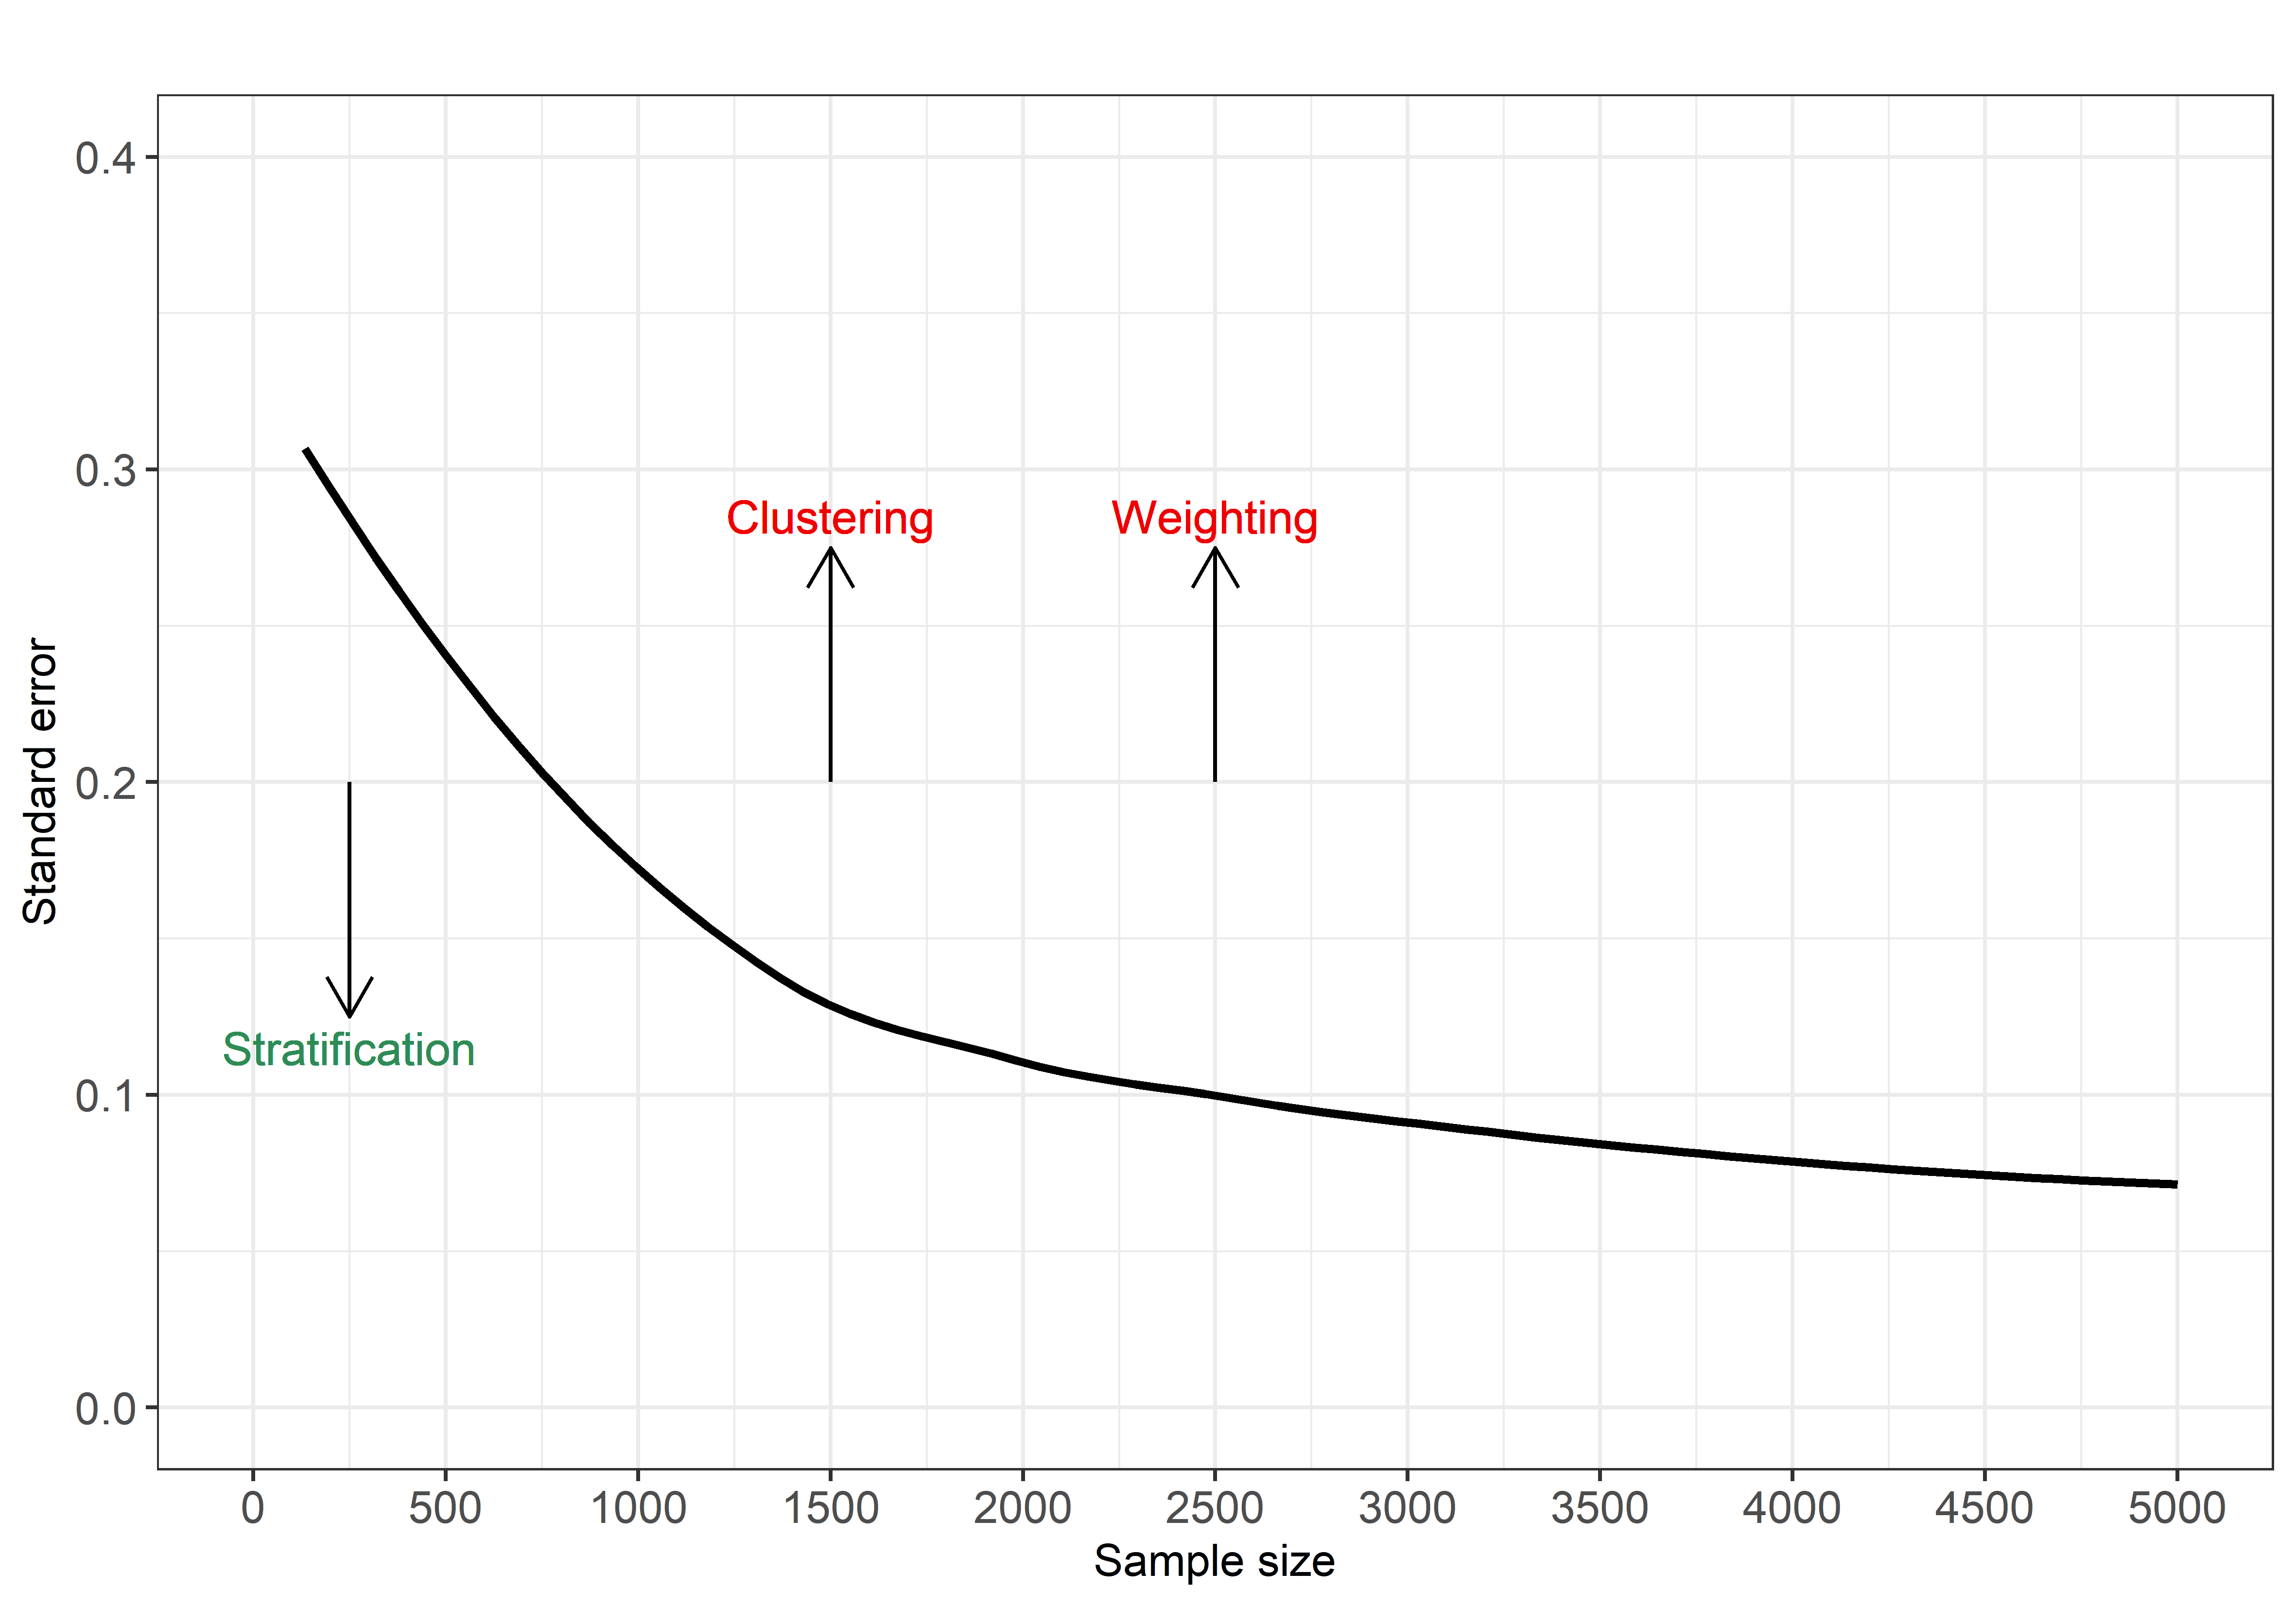
\includegraphics[scale = 0.09]{images/srs_se}
\caption{Standard error of $\widehat{\mu}$ under an SRS design and the effect of CSS design elements. Adaptation of a simulation in \citet{heeringa2017}.}
\label{fig:precision}
\end{figure}

The plotted curve is the simulated standard error of $\widehat{\mu}$ under an SRS design, where $\mu \sim \mathcal{N}(0, 5)$. In general, for an SRS of a given size, stratification results in increased precision, whilst clustering and weighting result in decreased precision \citep{heeringa2017}. We may wish to quantify the effect of these design elements on the precision of the estimate. In other words, we wish to know how the standard error obtained in a CSS, denoted $\text{SE}_{\text{css}}(\widehat{\mu})$, differs from the standard error that would be obtained in an SRS of equal sample size, denoted $\text{SE}_{\text{srs}}(\widehat{\mu})$ \citep{heeringa2017}. The ratio between the two variances is known as the design effect, $\text{D}^{2}(\widehat{\mu})$ \citep{kish1965}:

\begin{align}
\label{eq:true-design}
\text{D}^{2}(\widehat{\mu}) 		&=	\frac{\text{Var}_{\text{css}}(\widehat{\mu})}{\text{Var}_{\text{srs}}(\widehat{\mu})}			\\
\notag
\implies \text{D}(\widehat{\mu}) 		&=	\frac{\text{SE}_{\text{css}}(\widehat{\mu})}{\text{SE}_{\text{srs}}(\widehat{\mu})}
\end{align}

This is usually estimated empirically:

\begin{align}
\label{eq:empirical-design}
\text{d}^{2}(\widehat{\mu}) 				&= \frac{\text{var}_{\text{css}}(\widehat{\mu})}{\text{var}_{\text{srs}}(\widehat{\mu})}	\\
\notag
\implies \text{d}(\widehat{\mu}) 				&= \frac{\text{se}_{\text{css}}(\widehat{\mu})}{\text{se}_{\text{srs}}(\widehat{\mu})}	\\
\notag
\therefore \text{se}_{\text{css}}(\widehat{\mu}) 	&= \text{se}_{\text{srs}}(\widehat{\mu}) \times \text{d}(\widehat{\mu}) 		
\end{align}

We motivate the remainder of this section on design-based inference with artificial CSS data, consisting of systolic blood pressure (BP) measurements taken on 18 individuals and measured in mmHg. These data are presented in \autoref{table:data}.

\begin{longtable}{P{24mm}P{24mm}P{24mm}P{24mm}P{24mm}}
\toprule
Observation 		& BP ($y_i$) 				& Cluster ($\tau_i$)		& Stratum ($\gamma_i$)			& Weight ($w_i$) 		\\ \bottomrule
1           			& 116.9                                	& 1					& 1               					& 138          			\\ \hline
2           			& 109.1                                	& 1					& 1               					& 97         				\\ \hline
3           			& 110.7                                	& 1					& 1               					& 284         			\\ \hline
4           			& 112.5                                	& 2					& 1               					& 248       				\\ \hline
5           			& 114.6                                	& 2					& 1               					& 232        				\\ \hline
6           			& 117.7                             		& 2					& 1               					& 242          			\\ \hline
7           			& 117.2                        		& 3					& 2               					& 31	          			\\ \hline
8          			& 120.4                             		& 3					& 2               					& 275          			\\ \hline
9           			& 118.3                             		& 3					& 2               					& 58	          			\\ \hline
10           			& 125.9                             		& 4					& 2               					& 203          			\\ \hline
11           			& 122.7                             		& 4					& 2               					& 225          			\\ \hline
12           			& 124.9                             		& 4					& 2               					& 291          			\\ \hline
13           			& 129.2                             		& 5					& 3               					& 280          			\\ \hline
14           			& 126.5                             		& 5					& 3               					& 241          			\\ \hline
15           			& 131.2                             		& 5					& 3               					& 100          			\\ \hline
16           			& 134.3                             		& 6					& 3               					& 372          			\\ \hline
17           			& 127.9                             		& 6					& 3               					& 330          			\\ \hline
18           			& 135.1                             		& 6					& 3               					& 100          			\\ \bottomrule
\caption{Artificial CSS data of systolic BP in eight individuals.}
\label{table:data}
\end{longtable}

Note that this is a small sample size and some of the Gaussian assumptions may not hold true, for example in constructing confidence intervals (CIs). This data is only being used for illustrative purposes, and in real-life settings CSS data typically contain thousands of observations. 

Design-based analyses, also known as "distribution-free" or "nonparametric" approaches, make no assumptions of the underlying distribution for the variables of interest \citep{heeringa2017}. By considering the various aspects of survey design, the probability of a given sample being drawn from the target population is known. Therefore, it is possible to compute expectations and variances for variables of interest without specifying their distribution. The simplest example of design-based inference would be to assume the individuals in \autoref{table:data} were sampled under an SRS design. We can then compute summary statistics for $y$ in the usual manner (ignoring the FPC):

\begin{align}
\label{eq:srs-stats}
\bar{y}					&=	\frac{1}{n} \sum_{i = 1}^{n} (y_i) 					=	122.0			\\
\notag
\text{se}(\bar{y})			&=	\sqrt{ \frac{ \text{var}(y) }{ n } }						=	1.86			\\
\notag
95\%\text{ CI}				&=	\bar{y} \pm t_{0.975, 17} \times \text{se}(\bar{y})							\\
\notag
						&=	(118.0, 125.9)
\end{align}

By definition, the design effect for the estimate of $\bar{y}$ under an SRS design is 1.

\subsection{Clustering}

Clustered sampling is frequently employed in CSSs. It refers to when groups of individuals who typically share something in common are treated as single-unit clusters. Under an SRS design, we are effectively treating each observation as their own individual cluster of sample size 1. Clustering is implemented for several reasons \citep{heeringa2017}:

\begin{enumerate}
\item Clustering individuals by geographical region helps to reduce the cost of large-scale surveys by increasing efficiency of data collection and travel from location to location.
\item It might not be possible to identify individual elements of the target population at the initial stage, but it might be possible to identify cluster units within which they lie e.g., universities containing students of interest may be identified and then the universities visited to sample the individuals.
\item Intentionally clustering the sampling procedure allows for estimation of variance both between and within the variables of interest e.g., individuals within universities, universities within regions.
\end{enumerate}

Since these clusters contain individuals who have shared characteristics, this makes the individuals within a given cluster more homogenous than would be expected if they were sampled under an SRS framework i.e., we expect there is less information contained in a cluster of $n$ individuals, compared to $n$ individuals from an SRS \citep{heeringa2017}. This needs to be corrected for, which results in increased SEs for clustered samples. In order to correct the precision, we must quantify the degree of homogeneity that is observed within the clusters. A commonly used statistic to do so is known as the intraclass correlation, $\rho$ \citep{kish1965}. In order to gain some intuitive understanding of what $\rho$ is measuring, consider a sample of 100 university students which has been selected by randomly sampling 25 individuals studying 4 different subjects i.e., the samples are clustered by the subject studied. We ask them each two questions:

\begin{enumerate}
\item What was your average GCSE mark? We would expect individuals who are studying a subject with higher entry requirements to have a higher average GCSE mark than those studying subjects with lower entry requirements. Of course, the marks will not be identical for all individuals studying the same subject, but they will be highly correlated. In this case, we might assume $\rho$ to be in the range of 0.7.
\item How old is your oldest professor? Assuming all individuals studying a given subject have the same professors teaching them, then the same answer will be received from all 25 students within a cluster. In other words, we could have just asked one individual from each group the question and gained the same amount of information. In this case, $\rho = 1$.
\end{enumerate}

Let $y_{ij}$ be the $j^{\text{th}}$ observation in cluster $i$, let $J$ equal the number of clusters, let $K$ equal the number of observations per cluster, hence $JK$ is the total sample size. Without proof, we state a key result obtained by \citet{cochran1977}:

\begin{align}
\label{eq:cochran1}
\text{Var}_{\text{clus}}(\bar{y}) 		&=	\text{FPC} \times \frac{ \text{Var}(y) }{ JK } \times [1 + \rho (K - 1)]	\\
\notag
							&=	\text{FPC} \times \text{Var}(\bar{y}) \times [1 + \rho (K - 1)]
\end{align}

Where $\text{Var}_{\text{clus}}$ refers to the cluster-adjusted variance. Assuming $\text{FPC} \approx 1$, we obtain a good approximation for $\text{Var}_{\text{clus}}(\bar{y})$:

\begin{align}
\label{eq:cochran2}
\text{Var}_{\text{clus}}(\bar{y}) 		&\approx	\text{Var}(\bar{y})  \times [1 + \rho (K - 1)]   				\\
\notag
\implies \text{SE}_{\text{clus}}(\bar{y})	&\approx	\text{SE}(\bar{y}) \times \sqrt{ [1 + \rho (K - 1)] }		
\end{align}

Where $\rho$, the intraclass correlation, is the expectation of the ratio between the intraclass covariance and variance:

\begin{align}
\label{eq:cochran3}
\frac{ \mathbb{E}(y_{ij} - \bar{y})(y_{ik} - \bar{y}) }{ \mathbb{E}(y_{ij} - \bar{y}) ^ 2 }	=	\frac{2 \sum_{i} \sum_{j<k} (y_{ij} - \bar{y})(y_{ik} - \bar{y}) }{ (K - 1) (JK - 1) \text{Var}(y) }
\end{align}

The above equations hold true for the case where clusters contain equal sample sizes. The case of unevenly sized clusters requires adjustment of these equations, which will not be discussed here.

An interesting relationship arises when considering \autoref{eq:empirical-design} and \autoref{eq:cochran2} together, where we find \citep{heeringa2017}:

\begin{align}
\label{eq:deff-rho}
\text{d}^{2}(\bar{y})		\approx	1 + \rho (K - 1)
\end{align}

Note if $\rho$ is negative (which does occur, although infrequently) then $\text{d}^{2}(\bar{y}) < 1$ and there is actually an increase in precision due to clustering \citep{cochran1977}.   We also need to compute the cluster-adjusted estimate of $\bar{y}$, but it is easy to show that this simplifies to the SRS estimate. We define the cluster-level mean, $\bar{y}_{\tau}$:

\begin{align}
\label{eq:clust-mean}
\bar{y}_{\tau}	=	\frac{1}{J} \sum_{i} y_{i}
\end{align}

In order to obtain the individual-level mean, we need to divide the cluster-level mean by the number of observations per cluster:

\begin{align}
\label{eq:elmt-mean}
\bar{y}	=	\frac{\bar{y}_{\tau}}{K}	=	\frac{1}{JK} \sum_{i} y_{i}
\end{align}

Since $JK$ is the total sample size, we see that the estimate for $\bar{y}$ is identical to the SRS estimate. We can now use \autoref{eq:cochran2} and \autoref{eq:cochran3} to compute the cluster-adjusted standard error, $\text{SE}_{\text{clus}}(\bar{y})$, for the data in \autoref{table:data}:

\begin{align}
\label{eq:cluster-stats}
\bar{y}					&=		122.0												\\
\notag
\text{se}_{\text{clus}}(\bar{y})	&=		3.27												\\
\notag
95\%\text{ CI}				&=		\bar{y} \pm t_{0.975, 3} \times \text{se}_{\text{clus}}(\bar{y})		\\
\notag
						&=		(113.6, 130.3)
\end{align}

As expected, $\text{se}_{\text{clus}}(\bar{y}) > \text{se}(\bar{y})$. Note also the reduced degrees of freedom ($df$) for the quantile of the $t$-distribution, namely $df =  J - 1$, resulting in a much wider CI than the SRS estimate in \autoref{eq:srs-stats}. We also obtain an estimate for the design effect:

\begin{align}
\label{eq:cluster-deff}
\notag
\text{d}^{2}(\bar{y})			&=		\frac{\text{var}_{\text{clus}}(\bar{y})}{\text{var}_{\text{srs}}(\bar{y})}	\\
\notag
						&=		3.08													\\
\end{align}

It is estimated that clustering increases the variance of the estimate of $\bar{y}$ by a factor of 3.08.

\subsection{Stratification}

Strata are nonoverlapping subpopulations of the target population \citep{cochran1977}. If we take the target population of $N$ units and divide them into a set of $S$ subpopulations $\{ N_1, N_2, ..., N_S \}$, where:

\begin{align*}
N_1 + N_2 + ... + N_S = N
\end{align*}

We say there are $S$ strata. It is possible to randomly sample individuals or clusters from within each stratum, where the set of sampled observations are $\{ n_1, n_2, ..., n_S \}$. This is known as stratified random sampling \citep{cochran1977}. Stratification is utilised for several reasons:

\begin{enumerate}
\item The target population is often heterogenous. By dividing it into highly homogenous subpopulations, this increases the precision of population-level estimates.
\item If it is known there are certain subpopulations of interest, then stratification ensures a large enough sample size can be taken to obtain an appropriate degree of precision.
\item Individuals within the target population may live in vastly different conditions to one another, so different sampling approaches have to be taken to reach different subgroups.
\end{enumerate}

We assign each stratum a weight, $\alpha_{\gamma} = n_{\gamma} / n$, where $n_{\gamma}$ is the sample size in stratum $\gamma$ and $n$ is the total sample size. Hence, the estimate for the stratification-adjusted sample mean is effectively a weighted average \citep{cochran1977}:

\begin{align}
\label{eq:strat-mean}
\bar{y}	=	\sum_{\gamma = 1}^{S} \alpha_{\gamma} \bar{y}_{\gamma}
\end{align}

Where $\bar{y}_{\gamma}$ is the sample mean in stratum $\gamma$. In the situation where $\alpha_{\gamma}$ is the same for all strata, this is referred to as proportional allocation of the $n_{\gamma}$ and the estimate for $\bar{y}$ simplifies to the SRS estimate. The stratum-adjusted variance, $\text{Var}_{\text{strat}}(\bar{y})$, also takes the form of a weighted sum \citep{cochran1977}:

\begin{align}
\label{eq:strat-var}
\text{Var}_{\text{strat}}(\bar{y})	&=	\sum_{\gamma} \frac{ \alpha_{\gamma}^{2} \text{Var}(y_{\gamma}) }{ n_{\gamma} }	\\
\notag
						&=	\sum_{\gamma} \alpha_{\gamma}^{2} \text{Var}(\bar{y}_{\gamma})
\end{align}

We can now use \autoref{eq:strat-var} to compute the stratification-adjusted standard error, $\text{SE}_{\text{strat}}(\bar{y})$, for the data in \autoref{table:data}:

\begin{align}
\label{eq:strat-stats}
\bar{y}					&=		122.0												\\
\notag
\text{se}_{\text{strat}}(\bar{y})	&=		0.82												\\
\notag
95\%\text{ CI}				&=		\bar{y} \pm t_{0.975, 2} \times \text{se}_{\text{strat}}(\bar{y})		\\
\notag
						&=		(118.4, 125.5)
\end{align}

As expected, $\text{se}_{\text{strat}}(\bar{y}) < \text{se}(\bar{y})$. Note that the CI is not substantially narrower than the SRS estimate, but this is because $df = S - 1 = 2$ i.e., number of strata minus 1. Therefore, the quantile from the \emph{t}-distribution is relatively large. In real-life data, there are typically far more than just 3 strata, so the effect of changing the $df$ is minimal. As a result, the stratification-adjusted CIs will almost always be much narrower than the SRS CIs. We also obtain an estimate for the design effect:

\begin{align}
\label{eq:strat-deff}
\notag
\text{d}^{2}(\bar{y})			&=		\frac{\text{var}_{\text{strat}}(\bar{y})}{\text{var}_{\text{srs}}(\bar{y})}	\\
\notag
						&=		0.19													\\
\end{align}

It is estimated that stratification decreases the variance of the estimate of $\bar{y}$ by a factor of 0.19.

\subsection{Weighting}

In order to obtain unbiased population-level estimates, the survey sample must be related back to the target population. Weighting survey data allows for computation of statistics which are representative of the target population i.e., the estimates are expected to be the same as those which would have been obtained had the whole target population been sampled. In an approximate sense, sample weights can often be thought to be equivalent to the number of individuals in the target population who are represented by a given participant. Note that this is not exactly true because the precise methods for how the final analysis weights are calculated are highly nuanced. Given a set of final analysis weights, $w_{\text{final}}$, these are computed as \citep{heeringa2017}:

\begin{align}
\label{eq:final-wt}
w_{\text{final}} = w_{\text{sel}} \times w_{\text{nr}} \times w_{\text{ps}}
\end{align}

Where $w_{\text{sel}}$ is the reciprocal of the probability that an observation was sampled from the target population, $w_{\text{nr}}$ is a factor which accounts for survey nonresponse, and $w_{\text{ps}}$ is a poststratification factor. Computing each of these requires substantial methodological considerations by survey statisticians when designing a CSS. 

An unbiased estimator for the weighted average is well-defined:

\begin{align}
\label{eq:wt-mean}
\bar{y}	=	\frac{ \sum_{i} w_{i} y_{i} }{ \sum_{i} w_{i} }
\end{align}

Computation of the weight-adjusted variance, $\text{Var}_{\text{wt}}(\bar{y})$, is more complex and one commonly used formula is derived below:

\begin{align}
\label{eq:wt-var}
\text{Var}_{\text{wt}}(\bar{y})	&=	\text{Var}(\frac{ \sum_{i} w_{i} y_{i} }{ \sum_{i} w_{i} })			\\
\notag
						&=	\sum_{i} \text{Var}(\frac{ w_{i} y_{i} }{ \sum_{i} w_{i} })			\\
\notag
						&=	\text{Var}(y) \frac{ \sum_{i} w_{i}^{2} }{ (\sum_{i} w_{i})^{2} }
\end{align}

Note how in the case where the weights are all equal to 1, this reduces to the SRS estimate. It is easy to see this is a biased estimator as, when taking the sums of the variance, the covariances are assumed to be 0. In practice, almost all software will use Taylor series linearisation to estimate variance, which we implement below to calculate the weight-adjusted standard error, $\text{SE}_{\text{wt}}(\bar{y})$, for the data in \autoref{table:data}:

\begin{align}
\label{eq:wt-stats}
\bar{y}					&=		122.7												\\
\notag
\text{se}_{\text{wt}}(\bar{y})	&=		2.03												\\
\notag
95\%\text{ CI}				&=		\bar{y} \pm t_{0.975, 13.9} \times \text{se}_{\text{wt}}(\bar{y})	\\
\notag
						&=		(118.3, 127.0)
\end{align}

After accounting for weighting, the estimate for $\bar{y}$ no longer coincides with the SRS estimate. Note that $df \neq n - 1$, instead they become $\frac{ (\sum_{i} w_{i})^{2} }{ \sum_{i} w_{i}^{2} } - 1$.  We also obtain an estimate for the design effect:

\begin{align}
\label{eq:wt-deff}
\notag
\text{d}^{2}(\bar{y})			&=		\frac{\text{var}_{\text{wt}}(\bar{y})}{\text{var}_{\text{srs}}(\bar{y})}	\\
\notag
						&=		1.23													
\end{align}

It is estimated that weighting increases the variance of the estimate of $\bar{y}$ by a factor of 1.23.

\subsection{Joint effects}

Presented in \autoref{table:combined-eff} are a set of summary statistics showing the estimate of $\bar{y}$, its associated standard error, and the design effect, when accounting for each combination of the CSS design variables. There is also a fourth statistic of interest presented, which is known as the effective sample size ($n_{\text{eff}}$). This is closely related to the design effect and given as \citep{heeringa2017}:

\begin{align}
n_{\text{eff}}				&=		n_{\text{css}} / \text{d}^{2}(\bar{y})
\end{align}

Where $n_{\text{css}}$ is the sample size of the CSS and $\text{d}^{2}(\bar{y})$ is the design effect for the estimand of interest (in this case, $\bar{y}$). The effective sample size tells us the sample size which would be required under an SRS design in order to achieve the same precision as that obtained by the CSS design \citep{heeringa2017}. In other words, to say "the design effect is equal to 1.1" is the same as saying "the CSS of size $n = 1,000$ has an effective sample size $n_{\text{eff}} = 910$".

\begin{longtable}{P{30mm}P{22.5mm}P{22.5mm}P{22.5mm}P{22.5mm}}
\toprule
Design 	 			& $\bar{y}$ 				& $\text{se}(\bar{y})$			& $\text{d}^{2}(\bar{y})$		& $n_{\text{eff}}$			\\ \bottomrule
SRS          				& 122.0                        		& 1.86					& 1.00      					& 18		         			\\ \hline
Clustered           			& 122.0                        		& 3.27					& 3.08               				& 6						\\ \hline
Stratified          			& 122.0                         		& 0.82					& 0.19               				& 95						\\ \hline
Weighted           			& 122.7	                        		& 2.03					& 1.19               				& 16						\\ \hline
Clus + Strat           		& 122.0                     			& 1.22					& 0.43               				& 42						\\ \hline
Clus + Weight           		& 122.7	                       		& 3.34					& 3.22               				& 6						\\ \hline
Strat + Weight           		& 122.7	                         		& 1.11					& 0.35               				& 52						\\ \hline
All           				& 122.7	                       		& 1.17					& 0.39               				& 47						\\ \bottomrule
\caption{Design effects for all combinations of CSS design variables.}
\label{table:combined-eff}
\end{longtable}

From \autoref{table:combined-eff}, it can be seen that there is a constant trade-off between the decreased precision due to clustering and weighting versus the increased precision from stratification. After accounting for all three design variables, the design effect is 0.39, meaning there is a 61\% reduction in the variance of the estimate of  $\bar{y}$, relative to an SRS of the same size. In other words, the CSS of size 18 yields a precision equivalent to an SRS of size 47. It should be noted that this is actually a relatively uncommon scenario. With real-life data, the design effect tends to be > 1 as the effect of clustering "overwhelms" the effect of stratification. This is because it is difficult for those designing the survey to obtain a substantial reduction in variance through stratification, unless they have extensive covariate data on the target population prior to sampling \citep{heeringa2017}.

\section{Model-based inference}

Design-based analyses allow statisticians to make a wide range of inferences about the target population without assuming any underlying distribution for the variable of interest. The only knowledge required for design-based analysis is the known distribution for the probability of the CSS sample being chosen from the target population. However, there are times when design-based analyses may not be adequate for addressing the scientific question at hand. 

In particular, scenarios where the aim is to elucidate causality or, at the very least, assess the relationship between multiple variables, do not lend themselves well to an approach which is solely design-based. The investigator may be required to fit a statistical model which approximates the relationship between the variables of interest. This means assumptions must be made about the probability distribution of the variables, which is where model-based and design-based inference differ from one another. 

Consider the classical linear regression:

\begin{align*}
\label{eq:linear-reg}
Y \mid X \sim \mathcal{N}(\beta_{0} + \beta_{1} x, \sigma^{2})
\end{align*}

From this, the model is fully specified and the parameters are identifiable by a method such as ordinary least squares, maximum likelihood estimation (MLE), or the method of moments. Naturally, the question which arises is whether the parameters of a given statistical model can also be identified in the context of survey data. If so, this would be a powerful tool to infer the relationship between variables of interest in the target population.

\subsection{Logistic regression}

We start by briefly reviewing logistic regression under an SRS setting, for which the methodology is extremely well-established \citep{mccullagh1989}. Consider a binary variable denoted $Y_{i}$ and a vector of observed covariates denoted $\mathbf{x}_{i}$:

\begin{align}
\label{eq:logistic-expectation}
\mathbb{E}(Y_{i} \mid \mathbf{x}_{i}) = P(Y_{i} = 1) = \mu_{i}
\end{align}

Since $\mu_{i}$ is a probability, it is bounded in $[0, 1]$ and we require a way to map it to a linear predictor, which can take any value on the real line. Hence, we identify a link function $g(.)$, such that $g: \mu_{i} \rightarrow \mathbb{R}$:

\begin{align}
\label{eq:logistic-link}
g(\mu_{i}) = \text{log} \left( \frac{\mu_{i}}{1 - \mu_{i}} \right) = \mathbf{x}_{i}^{T} \bm{\beta}
\end{align} 

The above function is known as the logit function and it acts as the canonical link for a variable following the Binomial distribution. We can obtain predictions for $\mu_{i}$ by taking the inverse of $g(.)$, denoted $h(.)$, such that $h(.)$ has support on $(-\infty, \infty)$ and codomain bounded in $[0, 1]$:

\begin{align}
\label{eq:logistic-inverse}
\mu_{i} = h(\mathbf{x}_{i}^{T} \bm{\beta}) = \frac{ \text{exp}(\mathbf{x}_{i}^{T} \bm{\beta}) }{ 1 + \text{exp}(\mathbf{x}_{i}^{T} \bm{\beta}) }
\end{align} 

In order to estimate $\bm{\beta}$, an iterative algorithm will be used to maximise a likelihood of the form:

\begin{align}
\label{eq:logistic-likelihood}
\mathcal{L}(\bm{\beta} | \mathbf{x}_{i})		=	\prod_{i = 1}^{n} \left( \frac{ \text{exp}(\mathbf{x}_{i}^{T} \bm{\beta}) }{ 1 + \text{exp}(\mathbf{x}_{i}^{T} \bm{\beta}) } \right) ^ {y_{i}} \left( \frac{ 1 }{ 1 + \text{exp}(\mathbf{x}_{i}^{T} \bm{\beta}) } \right) ^ {1 - y_{i}}
\end{align}

Following this, the appropriate model diagnostics and goodness of fit metrics will be assessed to determine whether the model has been adequately specified.

\subsection{Pseudo-maximum likelihood}

The addition of survey design variables means that the standard MLE procedures described above are not feasible \citep{heeringa2017}. This is because the conventional MLE approach requires observations to be sampled independently, but the use of clustering and stratification means this is no longer true. In addition, the probability of each of the observations being sampled is not equal, hence the survey weights have to be accounted for to obtain parameter estimates which relate back to the target population. This results in the following psuedo-likelihood:

\begin{align}
\label{eq:logistic-pseudo}
\mathcal{L}^{*}(\bm{\beta} | \mathbf{x}_{i})		=	\prod_{i = 1}^{n} \left\{ \left( \frac{ \text{exp}(\mathbf{x}_{i}^{T} \bm{\beta}) }{ 1 + \text{exp}(\mathbf{x}_{i}^{T} \bm{\beta}) } \right) ^ {y_{i}} \left( \frac{ 1 }{ 1 + \text{exp}(\mathbf{x}_{i}^{T} \bm{\beta}) } \right) ^ {1 - y_{i}} \right\} ^ {w_{i}}
\end{align}

And the corresponding pseudo-log-likelihood:

\begin{align}
\label{eq:logistic-pseudo-log}
\ell^{*}(\bm{\beta} | \mathbf{x}_{i})			=	\sum_{i = 1}^{n} w_{i} \left\{ y_{i} \text{log} \left( \frac{ \text{exp}(\mathbf{x}_{i}^{T} \bm{\beta}) }{ 1 + \text{exp}(\mathbf{x}_{i}^{T} \bm{\beta}) } \right) + (1 - y_{i}) \text{log} \left( \frac{ 1 }{ 1 + \text{exp}(\mathbf{x}_{i}^{T} \bm{\beta}) } \right) \right\}
\end{align}

Where $w_{i}$ are the survey weights. The model parameters are typically estimated using a pseudo-MLE (PMLE) approach, which was bought to popularity by \citet{roberts1987}. Full derivation of the PMLE approach is highly technical and we briefly summarise some of the key points. Assume we are given a binary dependent variable, a binomial likelihood, strata which are indexed by $\gamma$, clusters within each stratum which are indexed by $\tau$, and observations within each cluster which are indexed by $i$. Then the PMLE approach for obtaining estimates of $\bm{\beta}$ and its corresponding covariance matrix require the following vector of estimating equations to be solved \citep{binder1983}:

\begin{align}
\label{eq:logistic-eqns}
\Psi(\bm{\beta}) 	&= \sum_{\gamma} \sum_{\tau} \sum_{i} w_{\gamma \tau i} \mathbf{D}_{\gamma \tau i}^{T} \left[ \left( h(\mathbf{x}_{\gamma \tau i}^{T} \bm{\beta}) \right) \left( 1 - h(\mathbf{x}_{\gamma \tau i}^{T} \bm{\beta}) \right) \right] ^ {-1} \left( y_{\gamma \tau i} - h(\mathbf{x}_{\gamma \tau i}^{T} \bm{\beta}) \right) \\
\notag
			&= \mathbf{0}	
\end{align}

Where $h(\mathbf{x}_{\gamma \tau i}^{T} \bm{\beta})$ is the inverse logit function described in \autoref{eq:logistic-inverse} and $\mathbf{D}_{\gamma \tau i}$ is the vector of partial derivatives:

\begin{align}
\label{eq:logistic-D}
\mathbf{D}_{\gamma \tau i} = \left[ \frac{ \partial h(\mathbf{x}_{\gamma \tau i}^{T} \bm{\beta}) }{ \partial \beta_{j} } \right] \forall j \in \{ 0, ..., p \}
\end{align}

In the case of a logistic regression model, this simplifies to a set of $p + 1$ estimating equations \citep{heeringa2017}:

\begin{align}
\label{eq:logistic-eqns-simple}
\Psi(\bm{\beta}) = \sum_{\gamma} \sum_{\tau} \sum_{i} w_{\gamma \tau i} \left( y_{\gamma \tau i} - h(\mathbf{x}_{\gamma \tau i}^{T} \bm{\beta}) \right) \mathbf{x}_{\gamma \tau i}^{T} = \mathbf{0}
\end{align}

Where $\mathbf{x}_{\gamma \tau i}^{T}$ is the column vector of the design matrix elements for observation $i$, within cluster $\tau$, within stratum $\gamma$. A solution to the above equations can be found using an iterative algorithm, such as the Newton-Raphson method, and $\hat{\bm{\beta}}$ is obtained. The PMLE estimator for $\bm{\beta}$ is consistent but biased, however the bias $\rightarrow 0$ as $n \rightarrow \infty$. Given that complex surveys typically have large sample sizes, this bias will usually be very close 0, hence not of great concern to survey statisticians \citep{heeringa2017}.

Obtaining the variance-covariance matrix of the parameter estimates is far more challenging. The most commonly used method is estimation by Taylor series linearisation, which was introduced by \citet{binder1983} and takes the form:

\begin{align}
\label{eq:variance-estimator}
\text{Var}(\hat{\bm{\beta}})		=		( \mathbf{J}^{-1} ) \text{Var}(\Psi(\hat{\bm{\beta}})) ( \mathbf{J}^{-1} )
\end{align}

Where $\mathbf{J}$ is the matrix of second derivatives of $\ell^{*}(\bm{\beta} | \mathbf{x}_{i})$ in \autoref{eq:logistic-pseudo-log}, with respect to the $\hat{\beta}_{j}$:

\begin{align}
\label{eq:logistic-J}
\mathbf{J} = - \left[ \frac{ \partial^{2} \ell^{*}(\bm{\beta} | \mathbf{x}_{i}) }{ \partial \beta_{j} \partial \beta_{k} } \right] \forall j,k \in \{ 0, ..., p \}
\end{align}

$\text{Var}(\Psi(\hat{\bm{\beta}}))$ is the variance-covariance matrix for the equations in \autoref{eq:logistic-eqns-simple}. Full details of how this matrix is estimated are extensive and not provided here, but can be found in \citet{binder1983}.

\subsection{Model diagnostics}

Assessing goodness of fit (GOF) for design-adjusted regression models is a much more complex task than assessing goodness of fit in an SRS setting. This is primarily because a pseudo-likelihood, rather than a true likelihood, is used to fit the model, meaning that many of the tests which rely on the results derived from MLE are no longer valid.

\subsubsection{Wald tests}

One of the most commonly used methods for assessing model fit under a CSS design is the use of Wald tests. Assume we have a set of parameters ($\bm{\hat{\beta}}$) and we wish to test the null hypothesis that some linear combination of these coefficients is equal to a certain value, where the linear transformation is given by multiplication of the matrix $\mathbf{C}$. The most common test we wish to carry out is to test whether $\mathbf{C} \bm{\hat{\beta}} = 0$. The Wald test statistic is given as \citep{heeringa2017}:

\begin{align}
\label{eq:wald}
X^{2}_{\text{Wald}} = (\mathbf{C} \bm{\hat{\beta}})^{T} [ \mathbf{C} \text{Var}(\hat{\bm{\beta}}) \mathbf{C}^{T} ] ^ {-1} (\mathbf{C} \bm{\hat{\beta}})
\end{align}

Where $\text{Var}(\hat{\bm{\beta}})$ is the variance-covariance matrix described in \autoref{eq:variance-estimator}. Under the null hypothesis, the distribution of the test statistic is known \citep{heeringa2017}:

\begin{align}
\label{eq:wald-distribution}
X^{2}_{\text{Wald}} \sim \chi^{2}_{q}
\end{align}

Where $q$ is equal to the rank of $\mathbf{C}$. Note that $X^{2}_{\text{Wald}}$ will typically be divided by its degrees of freedom to convert it into an $F$-statistic and various first- or second-order corrections will be applied to account for the sampling design. In addition, it may be of interest to individually test each of the variables to assess how they alter model fit. One nuance to bring up is that survey statisticians should be cautious with tests of single parameters, when that parameter is actually part of a categorical variable with several levels, as a single parameter test does not inform us on the significance of the variable as a whole \citep{heeringa2017}.

Whilst the Wald test can be easy to carry out and interpret, there are several drawbacks: (i) the test statistic is not invariant to non-linear transformations of the parameters, (ii) small sample behaviour for Wald tests can be poor, (iii) the matrix $\text{Var}(\hat{\bm{\beta}})$ often has an unstable inverse and, for large $q$, can be singular \citep{lumley2014}. Therefore, likelihood ratio tests are often preferable, as they mitigate the above drawbacks.

\subsubsection{Pseudo-likelihood ratio tests}

It is often of interest to compare models, particularly when one model is nested within another, in order to assess whether the inclusion of a given predictor(s) improves fit. Under an SRS design, this is typically done using a generalised likelihood ratio test:

\begin{align}
\label{eq:glrt}
\Lambda = -2[ \ell_{(0)}(\bm{\beta} | \mathbf{x}_{i}) - \ell_{(1)}(\bm{\beta} | \mathbf{x}_{i}) ]
\end{align}

Where $\ell_{(0)}(\bm{\beta} | \mathbf{x}_{i})$ is the log-likelihood for the the restricted model and $\ell_{(1)}(\bm{\beta} | \mathbf{x}_{i})$ is the log-likelihood for the full model. Under some regularity assumptions, the distribution of the test statistic is known \citep{wilks1938}:

\begin{align}
\label{eq:glrt-distribution}
\Lambda \sim \chi^{2}_{q}
\end{align}

Where $q$ is the number of extra parameters in the full model, compared to the restricted model. However, this does not hold true for the CSS design as the sample is not independent and identically distributed, so there is no likelihood function. Hence, \citet{lumley2014} propose a design-adjusted statistic to carry out a pseudo-likelihood ratio test (PLRT):

\begin{align}
\label{eq:plrt}
\Lambda^{*} = -2n[ \ell^{*}_{(0)}(\bm{\beta} | \mathbf{x}_{i}) - \ell^{*}_{(1)}(\bm{\beta} | \mathbf{x}_{i}) ]
\end{align}

Where $\ell^{*}_{(0)}(\bm{\beta} | \mathbf{x}_{i})$ and $\ell^{*}_{(1)}(\bm{\beta} | \mathbf{x}_{i})$ refer to the pseudo-log-likelihood in \autoref{eq:logistic-pseudo-log} for the restricted and full model, respectively. Under certain regularity conditions, the test statistic converges in distribution \citep{lumley2014}:

\begin{align}
\label{eq:plrt-distribution}
\Lambda^{*} \xrightarrow{\text{d}} \sum_{1}^{q} \delta_{i} Z_{i}^{2}
\end{align}

Where the $Z_{i} \overset{\mathrm{iid}}{\sim} \mathcal{N}(0, 1)$. Full details on how the $\delta_{i}$ are computed are not given here, but they are often termed "generalised design effects" and are obtained by calculating the eigenvalues for a specific covariance matrix \citep{rao1981, rao1984}. Typically, the Rao-Scott first-order correction is then applied, and the distribution of the corrected test statistic is known (for specific types of sampling design) \citep{rao1981, lumley2014}:

\begin{align}
\label{eq:glrt-distribution-correct}
\Lambda^{*} / \bar{\delta} \sim \chi^{2}_{q}
\end{align}

Where $\bar{\delta} = \frac{1}{q} \sum_{i} \delta_{i}$. Under the null hypothesis that the fit of the full model is not an improvement over the restricted model, the distribution in \autoref{eq:glrt-distribution-correct} holds true and this allows for assessment of whether inclusion of the $q$ additional variables were of benefit.

It may be of interest to note that there are several design-adjusted estimators of pseudo-$R^{2}$ for logistic regression models. However, even under an SRS design, it is recommended that pseduo-$R^{2}$ is not quoted as a measure of model fit, due to the fact that it does not have an intuitive interpretation, unlike the $R^{2}$ value for linear regression \citep{hosmer2000, heeringa2017}. For survey data, the value becomes even further removed from having any intuitive meaning as it is not based on a true likelihood function. For those who are interested in how pseudo-$R^{2}$ can be estimated under a complex sampling design, we refer readers to \citet{lumley2017}, where the design-adjusted Cox-Snell and Nagelkerke estimators are presented.

\subsubsection{Goodness of fit}

Both the Wald test and PLRT are essentially testing whether a complex model is an improvement over a more simplified one, but they are not technically informing us on how well the model fits the data. In fact, GOF for survey data is currently an active area of research, with options for survey data still being very limited. The fact that there is no true likelihood for survey data means that obtaining GOF indices is very difficult. Broadly speaking, GOF tests for logistic regression models under an SRS design can be divided into four groups \citep{liu2007}:

\begin{enumerate}
\item Tests of residuals e.g., tests of the deviance or Pearson residuals
\item Tests of smoothed residuals e.g., le Cessie and van Howelingen's test
\item Tests of predicted probabilities e.g., Hosmer-Lemeshow test 
\item Score tests e.g., Stukel's test
\end{enumerate}

Testing the deviance residuals as a measure of GOF was first proposed by \citet{nelder1972}. In the case of an SRS sample, the test requires that the sum of the deviance residuals are compared to a $\chi^{2}_{n-p}$ distribution as an approximate measure of GOF. It is worth noting the deviance residuals only follow a $\chi^{2}$ distribution if the model is correct and this test has rather strong assumptions, most of which do not hold true for survey data as the samples are not independent. Furthermore, \citet{hosmer1997} showed that $p$-value from these tests are often highly uninformative for binary data.

Tests of the smoothed residuals, such as that proposed by \citet{lecessie1995}, involve taking kernel estimates of the standardised residuals in order to smooth their distribution. This is then compared to the theoretical asymptotic distribution of the smoothed residuals. The fact that the samples are not independently distributed in survey data violates the assumptions of these tests. In addition, these tests require user-defined bandwidths for the kernel, and it is known that tests which involve user input for determining the test statistic are highly variable with regards to the resulting \emph{p}-value \citep{hosmer1997}.

Another possibility is to partition the observations into $k$ ordered groups based on their predicted probabilities (when $k = 10$ these are often referred to as "risk deciles") and a chi-squared test is carried out on these groups \citep{hosmer1980}. Again, due to the fact the samples are not independent and identically distributed, this test is not valid under a CSS design. However, at least two extensions of the Hosmer-Lemeshow test have been derived for survey data \citep{archer2006, shah2003}. The same problem arises where this test is outdated as it requires an arbitrary user-defined value for $k$, and this choice substantially affects whether the test yields a highly significant or insignificant result. In addition, the only design-adjusted Hosmer-Lemeshow test which has been implemented in statistical software is that proposed by \citet{archer2006}, and this version of the test is not valid for analyses which are using subsamples of the complex survey.

Score tests, whilst not strictly GOF tests, are still useful for detecting issues with model fit \citep{hosmer1997}. The most popular score test is that proposed by \citet{stukel1988}, which involves assuming the fitted model comes from a family of generalised logistic models that contain two additional parameters to modify behaviour on the tails of the probability curve. Stukel's score test is testing the null hypothesis that both of these additional parameters are equal to 0, hence the predicted probabilities will be symmetric about 0.5 and the tails will display a regular behaviour \citep{liu2007}. Deviations from this behaviour, particularly in the noncentral probability region, can be detected by the score test, indicating the model may be inappropriate. As they do not measure GOF in the traditional sense (i.e., how well the observed data follow the expected data), score tests are heavily underutilised, with virtually no theory on their applications to survey data.

\subsubsection{Discrimative performance}

Given the substantial limitations in assessing GOF, the question arises as to whether it is possible at all to assess the fit of the model. Another route which can be taken is to assess how well the model predicts the status of the binary dependent variable. \citet{hosmer2000} refers to this as the \emph{discrimination} of the model, whilst GOF is referred to as the \emph{calibration} of the model. Of course, it is entirely possible for a model to have extremely high discriminative performance whilst being poorly calibrated i.e., the model does not represent the true generative process but can classify observations very well. However, in the absence of any rigorous GOF tests for models fit under a CSS design, we will turn to discriminative performance as the metric of interest.

One of the most commonly used measures is the area under the curve for the receiver operating characteristic (AUCROC), also referred to as the C-statistic. The ROC curve is a plot of sensitivity against $1 - \text{specificity}$, where sensitivity is defined as the probability of correctly classifying a positive observation and specificity is the probability of correctly classifying a negative observation. The area under this curve is informative of a model's ability to discriminate observations, with a value closer to 1 indicating better discrimination. Whilst there are no strict values for what constitutes a "good" AUCROC value, \citet{hosmer2000} proposed the following ranges:

\begin{itemize}
\item 0.5: No discrimination
\item 0.7 to $\leq$ 0.8: Acceptable discrimination
\item 0.8 to $\leq$ 0.9: Excellent discrimination
\item $\geq$ 0.9: Outstanding discrimination 
\end{itemize}

Since the AUCROC is based on the predicted probabilities, it relies solely on the point estimates for the model parameters. This means that the clustering and stratification do not need to be adjusted for in order to obtain a design-adjusted estimate of the AUCROC, as it is only weighting which affects the point estimates. This is useful as there is extensive theory on how to compute a weighted AUCROC, which effectively allows us to obtain an AUCROC value that is unbiased under a CSS design.

\section{Summary}

Overall, we see that CSS data requires a number of theoretical considerations to be taken into account to facilitate methodologically sound analyses. Design-based analyses are extremely useful in that they can provide highly informative statistics for the target population whilst making no distributional assumptions. However, the nature of such analyses is typically restricted to descriptive summaries of the data and one most turn to model-based methods to infer relationships between different variables. Whilst this approach increases the breadth of scientific questions which can be probed, it also relies on a greater number of assumptions to hold true. Hence, for any analytical method, there is a constant trade-off between its flexibility and the strength of the underlying assumptions required. Therefore, analyses should be theoretically driven, based on domain-specific knowledge and using appropriate data sources, in order to stand a chance of yielding robust findings.